\subsection*{a)}

\section*{Antwort}

Ein \textbf{Kontrollflussgraph} ist ein wichtiges Hilfsmittel bei der Sourcecodeanalyse und hilft u.a. bei der Bestimmung der Anzahl der vorhandenen Anweisungen (Knoten, $n$) in  einer Methode sowie ihrer Verzweigungen (Kanten, $e$) untereinander.\\
Der für den geg. Quellcode ermittelte Kontrollflussgraph ist in Abbildung~\ref{fig:kontrollflussgraph} dargestellt.

\begin{figure}
    \centering
    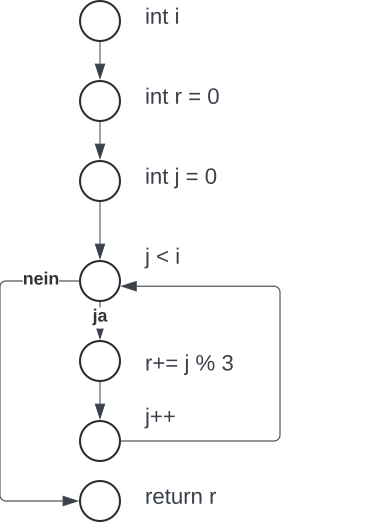
\includegraphics[scale=0.6]{chapters/aufgabe 7/img/kontrollflussgraph}
    \caption{Der Kontrollflussgraph zu Aufgabe 7 a). (Quelle: eigene )}
    \label{fig:kontrollflussgraph}
\end{figure}
